%% ID: phil_door_moments
%% TITLE: Pushing on a door
%% TYPE: question
%% QUESTIONTYPE:  scq
%% CONCEPTS: moments, forces
%% VIDEOS: 
%% LEVEL: 3
%% TOPIC: mechanics/statics
%% ORDER: 4

\begin{problem}[Phil_door_moments]
{\question{A woman pushes on a door at a distance \vari{d} from the hinges to open it. She pushes with a force of \vari{F} at an angle \vari{\theta} to the door. What is the moment acting about the hinges?}
\begin{enumerate}
	\item \choice[a]{\vari{Fd}}}
	\item \choice[b]{\vari{Fd\sin{\theta}}}
	\item \choice[c]{\vari{Fd\cos{\theta}}}
	\item \choice[d]{\vari{\frac{F\sin{\theta}}{d}}}
	\item \choice[e]{\vari{\frac{F\cos{\theta}}{d}}}
\end{enumerate}
}
{\textit{Created for the Rutherford School Physics Project by PS.}}
{\answer{\begin{figure} [h]
	\centering
	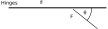
\includegraphics[width=0.4\textwidth]{../.././figures/Statics_door_moments.eps}
	\caption{}
	\label{fig:Statics_door_moments}
\end{figure}
The correct answer is (b). We can calculate the moment my multiplying the perpendicular component of the force by the distance from the pivot. The perpendicular component of the force is \vari{F\sin{\theta}} and the distance from the pivot is \vari{d}, therefore the moment is \vari{Fd\sin{\theta}}.}}
}
\end{problem}